%! TEX root = ./main.tex

\section{Algebras}
\begin{itemize}
    \item Overview \\
    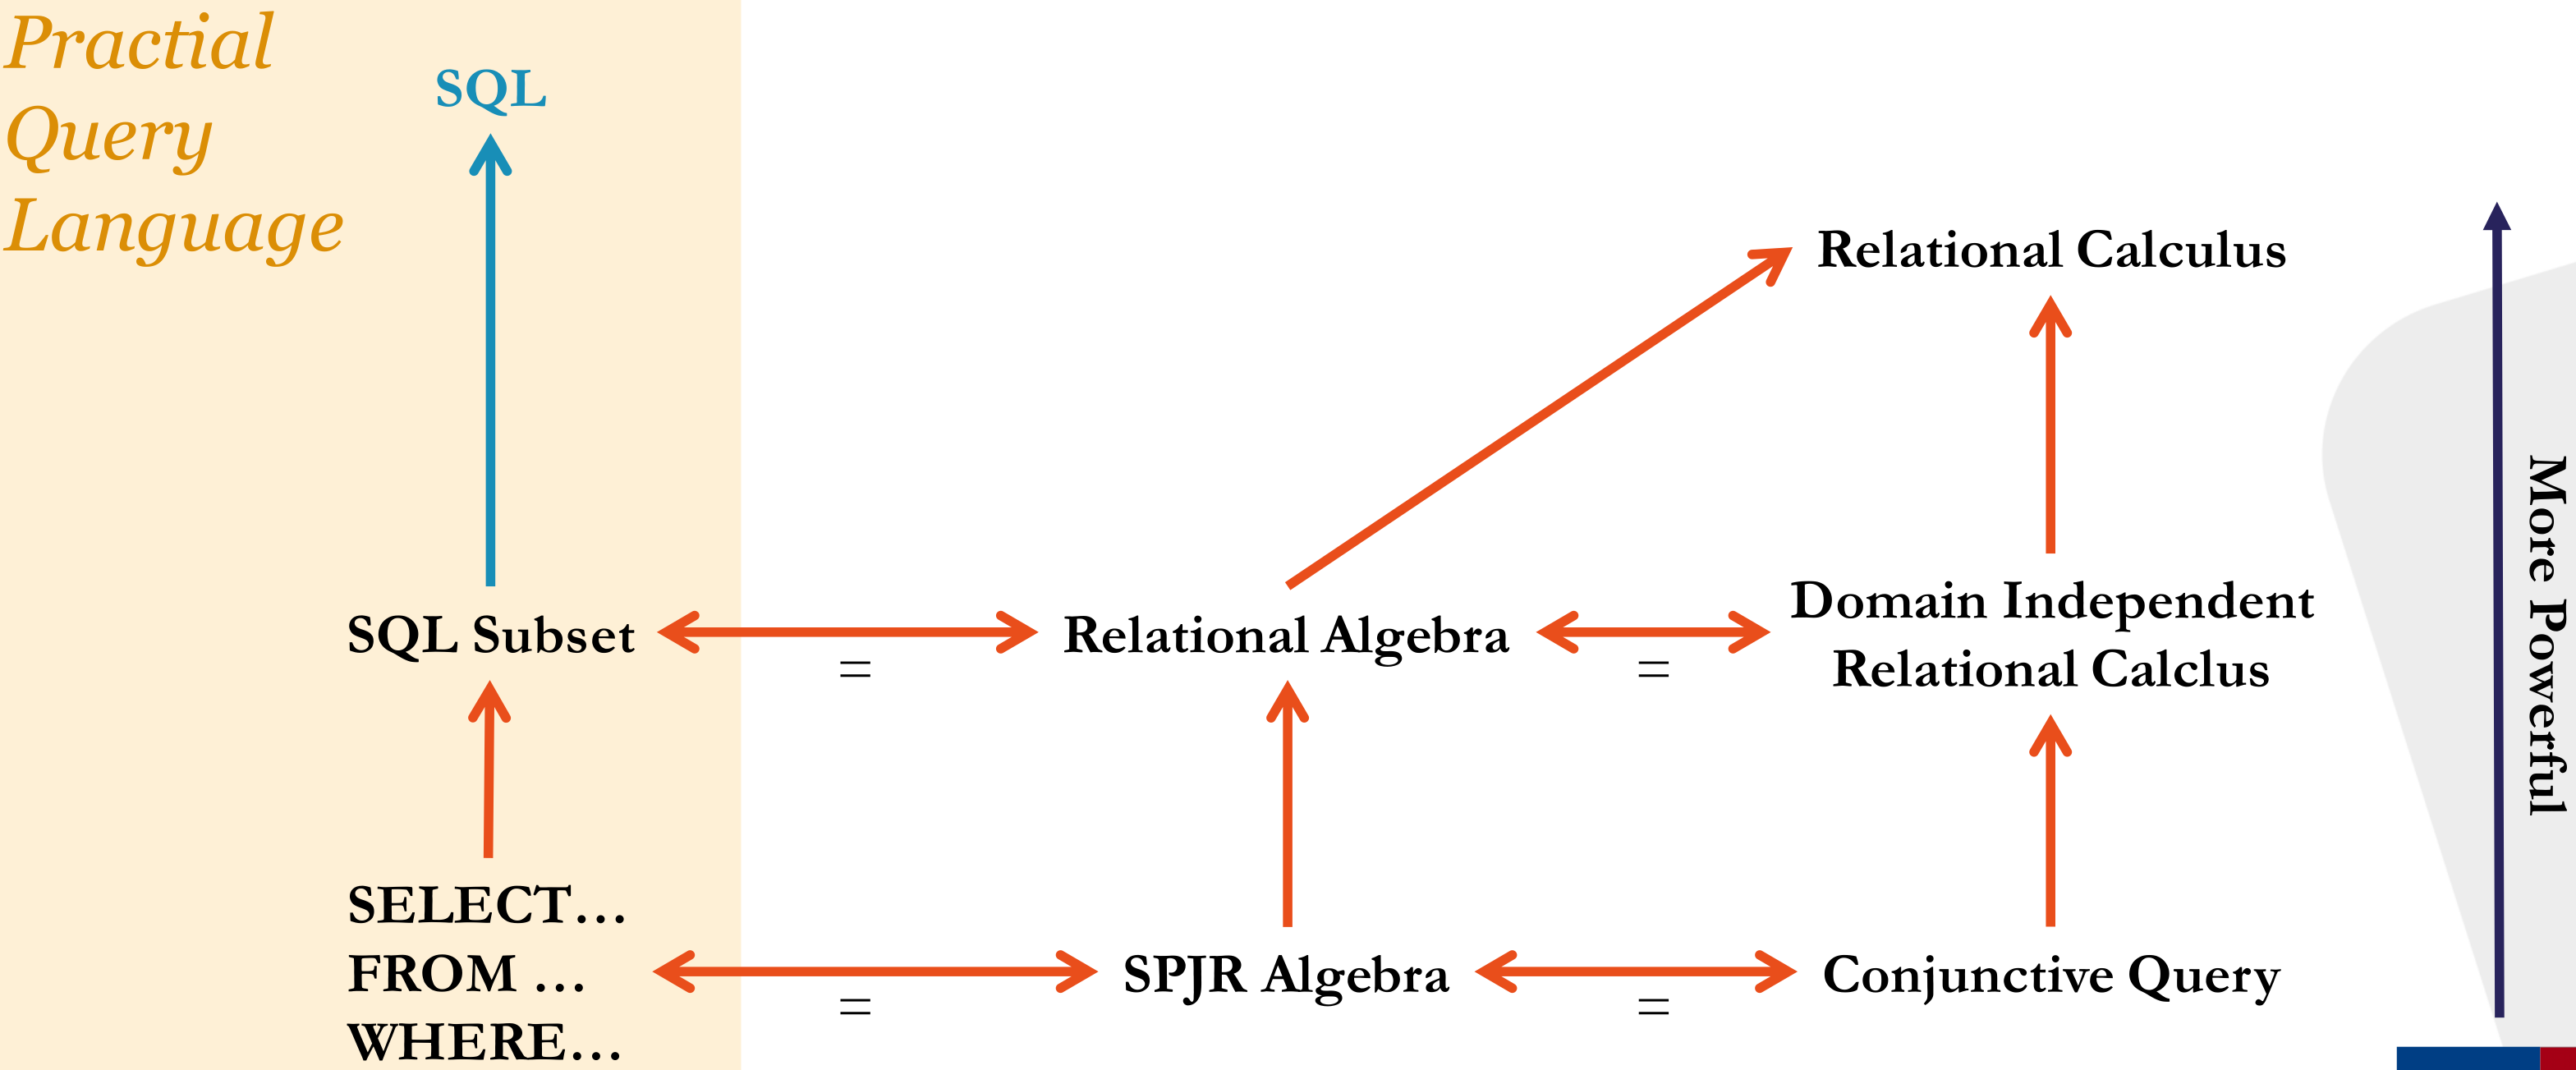
\includegraphics[width=0.8\textwidth]{./Figures/algebraOverview.png}
\end{itemize}

\section{Relational Algebra}
\begin{itemize}
    \item Imperative
        \begin{itemize}
            \item Say how we want it
            \item Different ways to implement the same query
        \end{itemize}
    \ides{Operators}
        \begin{itemize}
            \item Create a new relation $R'$ from one or two given relations $R_1, R_2$
            \ides{Union $\cup$:} 
                \begin{itemize}
                    \item $x \in R_1 \cup R_2 \iff x \in R_1 \lor x \in R_2$
                    \item Schema of both operands must match
                \end{itemize}
            \ides{Difference $-$:} 
                \begin{itemize}
                    \item $x \in R_1 - R_2 \iff x \in R_1 \land \neg (x \in R_2)$
                    \item Schema of both operands must match
                \end{itemize}
            \ides{Intersection $\cap$:} 
                \begin{itemize}
                    \item $x \in R_1 \cap R_2 \iff x \in R_1 \land x \in R_2$
                    \item Schema of both operands must match
                    \item Follows from $R_1 \cap R_2 = R_1 - (R_1 - R_2)$
                \end{itemize}
            \ides{Selection $\sigma$:}
                \begin{itemize}
                    \item $x \in \sigma_c (R) \iff x \in R \land c(x) = True$
                    \item Return tuples which satisfy a given condition $c$
                \end{itemize}
            \ides{Projection $\pi$}:
                \begin{itemize}
                    \item $\pi_{A_1,\dots,A_n} (R)$ keeps only columns $A_1, \dots A_n$
                \end{itemize}
            \ides{Cartesian Product $\times$:}
                \begin{itemize}
                    \item $(x, y) \in R_1 \times R_2 \iff x \in R_1 \land y \in R_2$
                    \item If $R_1$ and $R_2$ have columns in common renaming is required
                    \item Rarely used in practice
                \end{itemize}
            \ides{Renaming $\rho$:}
                \begin{itemize}
                    \item $\rho_{B_1, \dots, B_n} (R)$ changes the name of the attributes to $B_1, \dots B_n$
                    \item $\rho_S(R)$ changes the names of the attributes of $R$ to the one of $S$
                \end{itemize}
            \ides{Natural Join $\bowtie$:}
                \begin{itemize}
                    \item $R_1 (A, B) \bowtie R_2 (B, C) = \pi_{A, B, C} (\sigma_{R_1.B = R_2.B}(R_1 \times R_2))$
                            \begin{itemize}
                                \ides{No shared attributes:} Equivalent to cross product
                                \ides{All attributes shared:} Equivalent to intersect
                            \end{itemize}
                    \item Is associative
                \end{itemize}
            \ides{Theta Join $\bowtie_\theta$:}
                \begin{itemize}
                    \item $R_1 \bowtie_\theta R_2 = \sigma_\theta (R_1 \times R_2)$
                        \begin{itemize}
                            \item $\theta$ can be any kind of condition
                        \end{itemize}
                    \item Flavour
                        \begin{itemize}
                            \ides{Equi-Join:} $R_1 \bowtie_{A=B} R_2 = \sigma_{A=B} (R_1 \times R_2)$
                        \end{itemize}
                \end{itemize}
            \ides{Inner Join:}
                \begin{itemize}
                    \item Very similar to theta join with the difference that it keeps all matched columns
                        \begin{itemize}
                            \item I.e. matching columns are not collapsed into a single one
                        \end{itemize}
                \end{itemize}
            \ides{Outer Join:}
                \begin{itemize}
                    \ides{Left Outer Join ${\tiny \textifsym{d|><|}}$:} Natural join $\bigcup$ unmatched tuples from left operand
                    \ides{Right Outer Join ${\tiny \textifsym{|><|d}}$:} Natural join $\bigcup$ unmatched tuples from right operand
                    \ides{Full Outer Join ${\tiny \textifsym{d|><|d}}$:} Natural join $\bigcup$ unmatched tuples from left and right operand
                    \item Unmatched tuples from the left/right are extended with \verb+NULL+ in the columns which do not match
                \end{itemize}
            \ides{Semi Join:}
                \begin{itemize}
                    \ides{Left Semi Join $\ltimes$:} Tuples from left operand which match with any tuples from right operand
                        \begin{itemize}
                            \item $R_1(A_1, \dots, A_n) \ltimes R_2(B_1, \dots, B_2) = \Pi_{A_1, \dots, A_n}(R_1 \bowtie R_2)$
                        \end{itemize}
                    \ides{Right Semi Join $\rtimes$:} Tuples from right operand which match with any tuples from left operand
                \end{itemize}
            \ides{Relational Division $\div$:}
                \begin{itemize}
                    \item $A \div B = C$ where $C$ is the largest relation such that $B \times C \subseteq A$
                    \item Inverse of cross product
                \end{itemize}
        \end{itemize}
    \ides{Expression:} Composition of multiple operations
    \icon No infinite (recursive) queries
    \ides{Bags}
        \begin{itemize}
            \item Real DBMS use bag semantic
            \item Can have duplicates
            \item Difficult to extend RA to bags
                \begin{itemize}
                    \item Need to add new operators (duplicate elimination)
                \end{itemize}
        \end{itemize}
\end{itemize}

\section{Relational Calculus}
\begin{itemize}
    \item Declarative
        \begin{itemize}
            \item Say what we want
        \end{itemize}
    \item More powerful than RA
    \ides{Database Schema:} $S = (R_1, \dots, R_m), R_i$ is a relation
    \ides{Relation Schema:} $R(A_1:D_1, \dots , A_n:D_n)$
    \ides{Domain:} $\text{dom} = \bigcup_i D_i$
        \begin{itemize}
            \item Infinite set of constants
        \end{itemize}
    \ides{Instance of Relation $\mathbf{R(A_1:D_1, \dots, A_n:D_n)}$:} $I_R \subseteq \text{dom}^n$
        \begin{itemize}
            \item $I_R$ is finite
            \item Set of facts over the relation
        \end{itemize}
    \ides{Instance of DB $\mathbf{S(R_1, \dots , R_m)}$:} Function $\mathcal{I}$ that maps relation to an instance of that relation
        \begin{itemize}
            \item $\mathcal{I}: R_i \mapsto \mathcal{I}(R_i)$
            \item Finite
            \item Set of facts over all relations
        \end{itemize}
    \ides{Query $Q_\phi$:} Has the form $Q_\phi = \{(x_1, \dots, x_k) \mid \phi\}$
        \begin{itemize}
            \ides{$\mathbf{\phi}$:} First order formula (predicate) with free variables $x_1, \dots, x_k$
        \end{itemize} \todo{Full mathematical definition}
    \item Output of queries may be infinite
    \ides{Safe:} Query $Q_\phi$ which is finite for all $\mathcal{I}$
        \begin{itemize}
            \item Undecidable problem if query is safe
        \end{itemize}
    \ides{Domain Independent Relational Calculus:} Query whose result does not depend on the interpretation of the relation and not on the domain
    \ides{Active Domain:} $\text{adom}(Q_\phi, \mathcal{I}) = \text{all constaints in } Q_\phi \text{ and } \mathcal{I}$
    \ides{Conjunctive Query:} $\phi = \exists y_1, \dots, y_l (A_1 \wedge \dots \wedge A_m), Q_\phi = \{(x_1, \dots, x_n) \mid \phi \}, A_j$ is an atom
        \begin{itemize}
            \item Has many good properties
        \end{itemize}
    \ides{SPJR Algebra:} Relational algebra with only select, project, join and rename operators
\end{itemize}

